\documentclass[11pt,a4paper]{scrartcl}
\usepackage[utf8]{inputenc}
\usepackage[utf8]{inputenc}
\usepackage[ngerman]{babel}
\usepackage[T1]{fontenc}
\usepackage{amsmath}
\usepackage{amsfonts}
\usepackage{amssymb}
\usepackage{mathtools}
\usepackage{graphicx}
\usepackage{multirow}
\usepackage{fancyhdr}
\usepackage{float}
\pagestyle{fancy}
\usepackage[a4paper,
			bottom=1.7in,
			left=1.2in,
			right=1.2in,
			top=1.2in,
			headsep = 35pt]
	{geometry}
\usepackage{tikz}% for drawing automata etc
\usetikzlibrary{automata,arrows,chains,shapes.misc,scopes,petri,matrix,patterns}
%\usepackage[x11names]{xcolor}
%\usepackage[parfill]{parskip}
\usepackage{array}
%\usepackage{gslist}
%\usepackage{subfigure}
\usepackage{subcaption}
\usepackage{enumitem}
\usepackage{algpseudocode} %for pseudocode
\usepackage[siunitx,european,straightlabels,straightvoltages]{circuitikz} %draw Electrical Circuits
\usepackage[miktex]{gnuplottex}

\ctikzset{bipoles/text rotate/.initial=0,% <=new key
rotation/.style={\circuitikzbasekey/bipoles/text rotate=#1},% style for ease introduction in code
}

% code from pgfcircbipoles.sty
\makeatletter
\pgfcircdeclarebipole{}{\ctikzvalof{bipoles/ammeter/height}}{ammeter}{\ctikzvalof{bipoles/ammeter/height}}{\ctikzvalof{bipoles/ammeter/width}}{
    \def\pgf@circ@temp{right}
    \ifx\tikz@res@label@pos\pgf@circ@temp
        \pgf@circ@res@step=-1.2\pgf@circ@res@up
    \else
        \def\pgf@circ@temp{below}
        \ifx\tikz@res@label@pos\pgf@circ@temp
            \pgf@circ@res@step=-1.2\pgf@circ@res@up
        \else
            \pgf@circ@res@step=1.2\pgf@circ@res@up
        \fi
    \fi

    \pgfpathmoveto{\pgfpoint{\pgf@circ@res@left}{\pgf@circ@res@zero}}       
    \pgfpointorigin \pgf@circ@res@other =  \pgf@x  \advance \pgf@circ@res@other by -\pgf@circ@res@up
    \pgfpathlineto{\pgfpoint{\pgf@circ@res@other}{\pgf@circ@res@zero}}
    \pgfusepath{draw}

    \pgfsetlinewidth{\pgfkeysvalueof{/tikz/circuitikz/bipoles/thickness}\pgfstartlinewidth}

        \pgfscope
            \pgfpathcircle{\pgfpointorigin}{\pgf@circ@res@up} % change this if you want to touch the wires
            \pgfusepath{draw}       
        \endpgfscope    

    \pgftransformrotate{\ctikzvalof{bipoles/text rotate}}% <= magic line
    \pgfsetlinewidth{\pgfstartlinewidth}

    \pgfsetarrowsend{latex}
    \pgfpathmoveto{\pgfpoint{\pgf@circ@res@other}{\pgf@circ@res@down}}
    \pgfpathlineto{\pgfpoint{-1.06\pgf@circ@res@other}{1.06\pgf@circ@res@up}} % change this if you want to touch the wires
    %\pgfusepath{draw} % comment this if you don't need the diagonal arrow
    \pgfsetarrowsend{}


    \pgfpathmoveto{\pgfpoint{-\pgf@circ@res@other}{\pgf@circ@res@zero}}
    \pgfpathlineto{\pgfpoint{\pgf@circ@res@right}{\pgf@circ@res@zero}}
    %\pgfusepath{draw} % comment this if you don't need the diagonal arrow


    \pgfnode{circle}{center}{\textbf{A}}{}{}
}

% code from pgfcircbipoles.sty
\pgfcircdeclarebipole{}{\ctikzvalof{bipoles/voltmeter/height}}{voltmeter}{\ctikzvalof{bipoles/voltmeter/height}}{\ctikzvalof{bipoles/voltmeter/width}}{
    \def\pgf@circ@temp{right}
    \ifx\tikz@res@label@pos\pgf@circ@temp
        \pgf@circ@res@step=-1.2\pgf@circ@res@up
    \else
        \def\pgf@circ@temp{below}
        \ifx\tikz@res@label@pos\pgf@circ@temp
            \pgf@circ@res@step=-1.2\pgf@circ@res@up
        \else
            \pgf@circ@res@step=1.2\pgf@circ@res@up
        \fi
    \fi

    \pgfpathmoveto{\pgfpoint{\pgf@circ@res@left}{\pgf@circ@res@zero}}       
    \pgfpointorigin \pgf@circ@res@other =  \pgf@x  \advance \pgf@circ@res@other by -\pgf@circ@res@up
    \pgfpathlineto{\pgfpoint{\pgf@circ@res@other}{\pgf@circ@res@zero}}
    \pgfusepath{draw}

    \pgfsetlinewidth{\pgfkeysvalueof{/tikz/circuitikz/bipoles/thickness}\pgfstartlinewidth}

        \pgfscope
            \pgfpathcircle{\pgfpointorigin}{\pgf@circ@res@up} % change this if you want to touch the wires
            \pgfusepath{draw}       
        \endpgfscope    

    \pgftransformrotate{\ctikzvalof{bipoles/text rotate}}% <= magic line
    \pgfsetlinewidth{\pgfstartlinewidth}

    \pgfsetarrowsend{latex}
    \pgfpathmoveto{\pgfpoint{\pgf@circ@res@other}{\pgf@circ@res@down}}
    \pgfpathlineto{\pgfpoint{-1.06\pgf@circ@res@other}{1.06\pgf@circ@res@up}} % change this if you want to touch the wires
    %\pgfusepath{draw} % comment this if you don't need the diagonal arrow
    \pgfsetarrowsend{}


    \pgfpathmoveto{\pgfpoint{-\pgf@circ@res@other}{\pgf@circ@res@zero}}
    \pgfpathlineto{\pgfpoint{\pgf@circ@res@right}{\pgf@circ@res@zero}}
    %\pgfusepath{draw} % comment this if you don't need the diagonal arrow


    \pgfnode{circle}{center}{\textbf{V}}{}{}
}
\makeatother


\author{Alexander Halbarth}

\setlist[enumerate]{label=\alph*)}
%\setlist[itemize]{label=$\rightarrow$}


 \tikzset{
endbox/.style={pattern=crosshatch,minimum height=.8cm}}

%\partfont{\centering}
\newcommand\tab[1][1cm]{\hspace*{#1}}
\usepackage{framed, color}


\newcommand{\UE}{Übung 2}
\newcommand{\name}{Fragenkatalog zum Überprüfungsgespräch Elektrotechnische Grundlagen}
\title{\textbf{Fragenkatalog zum Überprüfungsgespräch Elektrotechnische Grundlagen Übungen für TI 2017 - \UE}}


\newcommand{\ul}[1]{\underline{#1}} % für unterstreichen von einzelnen Symbolen einfach \ul x - wenn man ein Wort unterstrichen will \ul{wort}
%\newcommand\sy[1]{{\underline{\ifmmode\mathtt{#1}\else\texttt{#1}\fi}}} % ähnlich wie \ul - verwendet aber andere Schriftart
%\newlistt\sys\sy{\hspace{1pt}}{}{}{^} % identisch zu \sy, \sys{wort} unterstreicht aber jeden Buchstaben einzeln und \sy{wort} unterstreicht das ganze Wort
% (sofern das Alphabet nur aus einzelnen Zeichen besteht ist \sys{wort} einfacher


%no line indent
\setlength\parindent{0pt}

\fancyhead[R]{\UE}
\fancyhead[L]{\name}
\fancyfoot[C]{\thepage}

\renewcommand{\footrulewidth}{0pt}
\renewcommand{\headrulewidth}{0.5pt}


\begin{document}
\maketitle
\textbf{Frage 1: Was machst Du gerade im Labor und welchen Sinn hat das?}\\
\textbf{Frage 2: Nenne die Grundgrößen der Elektrotechnik, deren Formelzeichen und Einheit.}\\
Spannung $U[$Volt $V]$, Strom $I[$Ampere $A]$, Widerstand $R[$Ohm $\Omega]$,Leistung $P[$Watt $W]$\\
\textbf{Frage 2: Elektrische Spannung: Nenne Definition (nicht über das Ohmsche Gesetz!), Formelzeichen und Einheit}\\
Die potentielle Energie(=Arbeit) die durch eine Ladungstrennung gespeichert wurde.\\
\textbf{Frage 2: Elektrischer Strom: Nenne Definition (nicht über das Ohmsche Gesetz!), Formelzeichen und Einheit}\\
Ladung eines Elektrons $Q_e=1,6 \cdot 10^{-19}C=1,6 \cdot 10^{-19}A\cdot s$\\
$\frac{6*10^{18}e^-}{1s}=\frac{As}{1s} \rightarrow 6*10^{18}$ Elektronen fließen durch einen Leiter pro Sekunde bei $1A$\\
\textbf{Frage 2: Elektrischer Widerstand: Nenne Definition (nicht über das Ohmsche Gesetz!), Formelzeichen und Einheit}\\
Ist eine Materialeigenschaft\\
Beispiel Kupfer $17m\Omega \cdot mm^2/m$\\
\textbf{Frage 2: Elektrische Leistung: Nenne Definition, Formelzeichen und Einheit}\\
Die in einer Zeitspannung umgesetzte elektrische Energie bezogen auf die Zeitspanne.\\
\textbf{Frage 2: Wie berechnet man die elektrische Leistung in einem Gleichstromkreis?}\\
$U=R \cdot I \rightarrow P=U \cdot I$\\
\textbf{Berechne die an einem Widerstand entstehende Leistung, wenn durch ihn bei einer Spannung von $2V$ ein Strom von $3A$ fließt.}\\
$6W$\\
\textbf{Frage 2: Welcher Phasenwinkel besteht zwischen Wechselspannung und Wechselstrom an einem idealen Kondensator?}\\
Die Spannung folgt dem Strom um $90^\circ=\pi/2$ nach. (eigentlich $-90^\circ$)\\
\textbf{Welcher Phasenwinkel besteht zwischen Wechselspannung und Wechselstrom an einer idealen Induktivität?\\
(Die Vorzeichen brauchen nicht explizit angegeben zu werden, müssen aber verglichen werden).}\\
Der Strom folgt der Spannung nach um $90^\circ=\pi/2$ nach. (eigentlich $+90^\circ$)\\
\textit{Gehen in entgegengesetzte Richtungen!}\\
\textbf{Frage 2: Formuliere das ohmsche Gesetz.}\\
$U=R*I$\\
\textbf{Berechne den Widerstand, wenn bei einem Strom von $3A$ eine Spannung von $3V$ abfällt.}\\
\textbf{Frage 2: Berechne den Strom, wenn an einem Widerstand von $5\Omega$ eine Spannung von $10V$ abfällt.}\\
\textbf{Frage 2: Berechne die Spannung, wenn durch einen Widerstand von $10\Omega$ ein Strom von $5A$ fließt. }\\
\textbf{Frage 2: Formuliere die Kirchhoffschen Regeln.}\\
\textbf{Auf welchem physikalischen Grundprinzip beruhen diese?}\\
\textit{Energieerhaltung}\\
Maschenregel: Summe aller Spannungen muss 0 ergeben.\\
Knotenregel: Summe aller Ströme muss 0 ergeben.\\
\textbf{An einem Spannungsteiler liegen $9V$. Am oberen Widerstand liegen $6V$ an.}\\
\textbf{Berechne die Spannung am unteren Widerstand.}\\
\textbf{Frage 2: In einen Stromknoten mit drei Leitungen fließen aus einer Leitung $2A$ hinein und aus einer anderen Leitung $3A$ hinein. Was geschieht in der dritten Leitung?}\\
\textbf{Frage 2: Nenne die Zehnerpotenzen zu den SI - Präfixen Nano, Milli und Mikro. Nenne die SI - Präfixe zu: $10^3, 10^6, 10^9$}\\
\begin{tabular}{|l|l|l|}
\hline
\textbf{Präfix} & \textbf{Zeichen} & \textbf{Faktor}\\
\hline\hline
Piko   & p  & $10^{-12}$\\
\hline
Nano   & n  & $10^{-9}$\\
\hline
Mikro  & $\mu$ & $10^{-6}$\\
\hline
Milli  & m  & $10^{-3}$\\
\hline
Zenti  & c  & $10^{-2}$\\
\hline
Dezi   & d  & $10^{-1}$\\
\hline\hline
Deka   & da & $10^{1}$\\
\hline
Hekto  & h  & $10^{2}$\\
\hline
Kilo   & k  & $10^{3}$\\
\hline
Mega   & M  & $10^{6}$\\
\hline
Giga   & G  & $10^{9}$\\
\hline
Tera   & T  & $10^{12}$\\
\hline
\end{tabular}\\
\newpage
\textbf{Frage 3: Skizziere einen Operationsverstärker.}\\
\begin{center}
\begin{circuitikz} \draw
			node[op amp]{};
\end{circuitikz}
\end{center}

\textbf{Gib seine Übertragungsfunktion an.}
\begin{center}
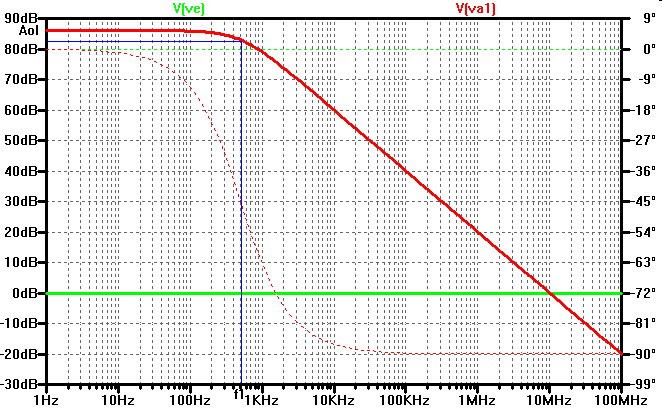
\includegraphics[width=7cm]{OPV_Uebertragung.png}
\end{center}
Tiefpassverhalten: Verstärkung ca $80dB=1000-fache$ Verstärkung, Grenzfrequenz ca $1kHz$

\textbf{Frage 3: Skizziere die Schaltung eines Operationsverstärkers als invertierender Verstärker.}
\begin{center}
\begin{circuitikz} 
	\draw (3.5,1.5) node[op amp] (OPV) {};
	\draw let \p1=(OPV.+) in (\x1,0) node [rground] (G2) {} -- (OPV.+);
	\draw (0,0) node [rground] (G1) {};
	\draw let \p1=(OPV.-),\p2=(OPV.out) in 
		(0,0) to[V<=$U_{in}$] (0,\y1)
						to[R=$R_1$,i_>=$I$,-*] (2,\y1)
						-- (OPV.-)
						(2,\y1) -- (2,3)
						to[R=$R_2$] (\x2,3)
						to[short,-*] (OPV.out)
						to[short,-o] ++(1,0)
						node[anchor=west] {$U_{out}$};
\end{circuitikz}
\end{center}
\textbf{Leite dessen Übertragungsfunktion aus den Kirchhoffschen Regeln ab.}\\
$U_{out}=-I \cdot R_2=-\frac{U_{in}}{R_1}\cdot R_2=-U_{in}\cdot \frac{R_2}{R_1}$

\textbf{Frage 3: Skizziere die Schaltung eines Operationsverstärkers als nichtinvertierender Verstärker.}
\begin{center}
\begin{circuitikz} 
	\draw (2,1.5) node[op amp, yscale=-1] (OPV) {};
	\draw (0,0) node [rground] (G1) {};
	\draw let \p1=(OPV.+),\p2=(OPV.out) in 
		(0,0) to[V<=$U_{in}$,i^>=$I$] (0,\y1)
						-- (OPV.+);
	\draw let \p1=(OPV.-),\p2=(OPV.out) in 
	  (OPV.-)   -- (\x1,0) 
						  to[short,-*] (\x2,0)
						  to[R=$R_1$] (\x2,-1.5)
						  node [rground] {}
		(OPV.out) to[R=$R_2$,-*] (\x2,0)
		(OPV.out) to[short,-o] ++(1,0)
						  node[anchor=west] {$U_{out}$}
		(\x2,0)   to[short,-o] ++(1,0)
							node[anchor=west] {$U_{in}$};
\end{circuitikz}
\end{center}
\textbf{Leite dessen Übertragungsfunktion aus der Spannungsteilerregel ab.}\\
$\dfrac{U_{out}}{U_{in}}=\dfrac{R_2+R_1}{R_1} \Rightarrow U_{out}=U_{in}\cdot \left(1+\dfrac{R_2}{R_1}\right)$

\textbf{Frage 3: Skizziere die Schaltung eines Operationsverstärkers als invertierender Schmitt Trigger.}
\begin{center}
\begin{circuitikz} 
	\draw (2,1.5) node[op amp] (OPV) {};
	\draw (0,0) node [rground] (G1) {};
	\draw let \p1=(OPV.-),\p2=(OPV.out) in 
		(0,0) to[V<=$U_{in}$,i^>=$I$] (0,\y1)
						-- (OPV.-);
	\draw let \p1=(OPV.+),\p2=(OPV.out) in 
	  (OPV.+)   -- (\x1,0) 
						  to[short,-*] (\x2,0)
						  to[R=$R_1$] (\x2,-1.5)
						  node [rground] {}
		(OPV.out) to[R=$R_2$,-*] (\x2,0)
		(OPV.out) to[short,-o] ++(1,0)
						  node[anchor=west] {$U_{out}$}
		(\x2,0)   to[short,-o] ++(1,0)
							node[anchor=west] {$U_{in}$};
\end{circuitikz}
\end{center}
\textbf{Woran erkennst Du, dass es sich um einen Schmitt Trigger und nicht um einen linearen Verstärker handelt?}\\
An der Mitkopplung am Plus Eingang.

\textbf{Frage 3: Operationsverstärkers als invertierender Schmitt Trigger:\\
Dessen Ausgangsspannungsbereich beträgt $\pm 10V$.\\
Dimensioniere die beiden Widerstände so, dass sich die Ausschaltspannung zu $+5V$ und die Einschaltspannung zu $-5V$ ergibt.}\\
Sie müssen gleich groß sein. (Spannungsteiler)

\textbf{Frage 3: Skizziere die Schaltung eines Operationsverstärkers als nichtinvertierender Verstärker. Der Operationsverstärker wird als ideal betrachtet.}
\begin{center}
\begin{circuitikz} 
	\draw (2,1.5) node[op amp] (OPV) {};
	\draw (0,0) node [rground] (G1) {};
	\draw let \p1=(OPV.-),\p2=(OPV.out) in 
		(0,0) to[V<=$U_{in}$,i^>=$I$] (0,\y1)
						-- (OPV.-);
	\draw let \p1=(OPV.+),\p2=(OPV.out) in 
	  (OPV.+)   -- (\x1,0) 
						  to[short,-*] (\x2,0)
						  to[R=$R_1$] (\x2,-1.5)
						  node [rground] {}
		(OPV.out) to[R=$R_2$,-*] (\x2,0)
		(OPV.out) to[short,-o] ++(1,0)
						  node[anchor=west] {$U_{out}$}
		(\x2,0)   to[short,-o] ++(1,0)
							node[anchor=west] {$U_{in}$};
\end{circuitikz}
\end{center}
\textbf{Gib den Eingangs‐ und Ausgangswiderstand dieser Schaltung an. Begründe Deine Darstellung!}\\
Eingangswiderstand ist unendlich\\
Ausgangswiderstand ist 0

\textbf{Frage 3: Skizziere die Schaltung eines Operationsverstärkers als invertierender Verstärker. Der Operationsverstärker wird als ideal betrachtet.}
\begin{center}
\begin{circuitikz} 
	\draw (3.5,1.5) node[op amp] (OPV) {};
	\draw let \p1=(OPV.+) in (\x1,0) node [rground] (G2) {} -- (OPV.+);
	\draw (0,0) node [rground] (G1) {};
	\draw let \p1=(OPV.-),\p2=(OPV.out) in 
		(0,0) to[V<=$U_{in}$,i^>=$I$] (0,\y1)
						to[R=$R_1$,-*] (2,\y1)
						-- (OPV.-)
						(2,\y1) -- (2,3)
						to[R=$R_2$] (\x2,3)
						to[short,-*] (OPV.out)
						to[short,-o] ++(1,0)
						node[anchor=west] {$U_{out}$};
\end{circuitikz}
\end{center}
\textbf{Gib den Eingangs‐ und Ausgangswiderstand dieser Schaltung an. Begründe Deine Darstellung!}\\
Eingangswiderstand ist $R_1$\\
Ausgangswiderstand ist 0

\textbf{Frage 4: Ein Operationsverstärker ist als nichtinvertierender Verstärker geschalten.\\
Skizziere den Verlauf der Verstärkung dieser Schaltung als Funktion der Frequenz (doppelt logarithmischer Maßstab).\\
Zeichne ein, welche maximale Verstärkung die Schaltung bei $0.1f_g$, $1f_g$, $10f_g$, $100f_g$ haben kann. ($f_g = $ Grenzfrequenz).}\\
\begin{center}
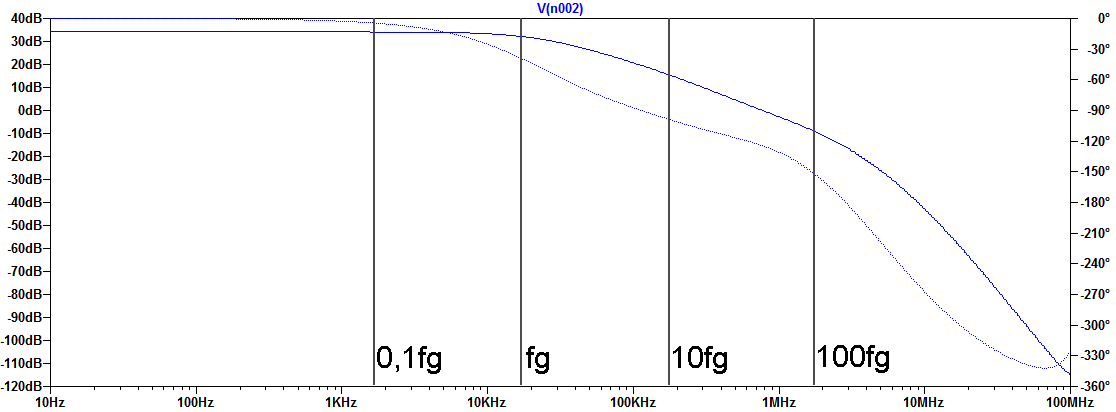
\includegraphics[width=14cm]{Nichtinvt_OPV_fg.png}
\end{center}

\textbf{Frage 4: Ein Operationsverstärker ist als nichtinvertierender Verstärker geschalten. Der Gegenkopplungswiderstand hat $9k\Omega$, der Widerstand zur Masse $1k\Omega$.
Der Operationsverstärker hat eine Verstärkung von $80dB$ bei Gleichspannung und eine Grenzfrequenz von $1kHz$.}\\
\textbf{Bestimme die Gleichspannungsverstärkung der \textit{Schaltung} und die maximale Frequenz, bei der diese Verstärkung noch erreicht wird.}\\
$U_{out}=U_{in} \cdot \left( 1+ \frac{R_2}{R_1} \right)= 1 \cdot \left( 1+ \frac{9k}{1k} \right)=10$\\
Eine 10 fache Verstärkung ($20 dB$) die Verstärkung wird bis knapp vor der Grenzfrequenz noch erreicht.

\textbf{Frage 4: Ein Operationsverstärker ist als nichtinvertierender Verstärker geschalten. Der Gegenkopplungswiderstand hat $9k\Omega$, der Widerstand zur Masse $1k\Omega$.
Der Operationsverstärker hat eine Verstärkung von $80dB$ bei Gleichspannung und eine Grenzfrequenz von $1kHz$.}\\
\textbf{Du legst an den Eingang eine $1kHz$ Rechteckspannung. Wird diese in akzeptabler Weise übertragen? Begründe Deine Entscheidung!}\\
Nein da sie bereits um $3dB$ Abgeschwächt wird.\\
\textbf{Du legst an den Eingang eine $1MHz$ Rechteckspannung. Wird diese in akzeptabler Weise übertragen? Begründe Deine Entscheidung!}\\
Nein da sie abgeschwächt wird.\\
\textbf{Frage 4: Ein Operationsverstärker ist als invertierender Schmitt Trigger geschalten. Der Operationsverstärker hat eine Verstärkung von $80dB$ bei Gleichspannung und eine Grenzfrequenz von $1kHz$. Die Schaltpunkte sind $\pm 1V$.}\\
\textbf{Du legst an den Eingang eine $10Hz$ Sinusspannung mit $\pm 10V$ Amplitude. Skizziere Eingangs- und Ausgangsspannungen als Funktion der Zeit. Begründe Deine Entscheidung!}\\
		\begin{figure}[H]
			\centering
			\begin{gnuplot}[terminal=pdf]
            set sample 1000
            set xlabel 't'
            set ylabel 'U'
						set label " 1" at 0.01,1.8
						set label "-1" at 0.01,-1.8
						set arrow 1 from 0,1 to 0.2,1 nohead filled lc "grey"
						set arrow 2 from 0,-1 to 0.2,-1 nohead filled lc "grey"
						Uout(t)= t<=0?0:Uin(t-0.001)<1&&Uin(t)>1?-10:Uin(t-0.001)>-1&&Uin(t)<-1?10:Uin(t)<1&Uin(t)>-1?Uout(t-0.001):Uin(t)>-1?-10:10
						Uin(t)=10*sin(20*pi*t)
            plot [0:0.2] [-15:15] Uin(x), Uout(x)
        \end{gnuplot}
			\end{figure}
\textbf{Du legst an den Eingang eine $10MHz$ Sinusspannung mit $\pm 10V$ Amplitude. Skizziere Eingangs- und Ausgangsspannungen als Funktion der Zeit. Begründe Deine Entscheidung!}\\
Kein Ausgang mehr, da Grenzfrequenz weit überschritten!

\newpage
\textbf{Frage 5: Ein Operationsverstärker ist als invertierender Integrator geschalten. Skizziere die Schaltung und gib die Übertragungsfunktion an.}\\
\begin{center}
\begin{circuitikz} 
	\draw (3.5,1.5) node[op amp] (OPV) {};
	\draw let \p1=(OPV.+) in (\x1,0) node [rground] (G2) {} -- (OPV.+);
	\draw (0,0) node [rground] (G1) {};
	\draw let \p1=(OPV.-),\p2=(OPV.out) in 
		(0,0) to[V<=$U_{in}$,i^>=$I$] (0,\y1)
						to[R,-*] (2,\y1)
						-- (OPV.-)
						(2,\y1) -- (2,3)
						to[C] (\x2,3)
						to[short,-*] (OPV.out)
						to[short,-o] ++(1,0)
						node[anchor=west] {$U_{out}$};
	\draw (OPV.out) node[inputarrow, xscale=-1, xshift=2.5mm] (I) {}
									node[below of = I, yshift=7mm] {$I$};
\end{circuitikz}
\end{center}
\begin{itemize}
	\item \textbf{Die Eingangsspannung beträgt konstant $+1V$. Zu Beginn des Versuchs ist die Ausgangsspannung $0V$. Skizziere den Verlauf der Ausgangsspannung über die Zeit.}
	\subitem $U_{out}(t)=-\frac{1}{R\cdot C}\cdot \int U_{in}(t)dt=-\frac{1}{R\cdot C}\cdot t$
			\begin{figure}[H]
				\centering
				\begin{gnuplot}[terminal=pdf]
            set sample 1000
            set xlabel 't'
            set ylabel 'U'
						set label "-1/RC" at -0.4,-0.5 textcolor lt 2
						set arrow 1 from -0.5,-0.5 to -0.45,-0.5 nohead filled lt 2
						Uout(t)=t<=0?0:-0.5*t
						Uin(t)=t<=0?0:1
            plot [-0.5:5] [-3:2] Uin(x), Uout(x)
        \end{gnuplot}
			\end{figure}
			\newpage
	\item \textbf{Die Eingangsspannung ist eine Rechteckspannung $\pm 10V$, beginnend mit der steigenden Flanke. Zu Beginn des Versuchs ist die Ausgangsspannung $0V$. Skizziere den Verlauf von Eingangs- und Ausgangsspannung über die Zeit.}
		\begin{figure}[H]
			\centering
			\begin{gnuplot}[terminal=pdf]
            set sample 1000
            set xlabel 't'
            set ylabel 'U'
						set label "-1/RC" at 0.1,-5 textcolor lt 2
						set arrow 1 from 0,-5 to 0.05,-5 nohead filled lt 2
						Uout(t)=-5*(t<=0?0:ceil(t)%2==1?t+(floor(t)):-t-(floor(t)))+(t<0?0:ceil(t)%2==0?-1:1)*10*floor(t)-(t<0?0:ceil(t)%2==0?5:0)
						Uin(t)=t<=0?0:ceil(t)%2==0?10:-10
            plot [0:10] [-12:12] Uin(x), Uout(x)
        \end{gnuplot}
			\end{figure}
	\item \textbf{Die Eingangsspannung ist Sinusspannung ($1V_{PP}$), beginnend mit 0V steigende Flanke. Zu Beginn des Versuchs ist die Ausgangsspannung $0V$. Skizziere den Verlauf von Eingangs- und Ausgangsspannung über die Zeit.}
		\begin{figure}[H]
			\centering
			\begin{gnuplot}[terminal=pdf]
            set sample 1000
            set xlabel 't'
            set ylabel 'U'
						set label "-1/RC" at 0.1,-0.7 textcolor lt 2
						set arrow 1 from 0,-0.7 to 0.05,-0.7 nohead filled lt 2
						Uout(t)=0.7*cos(t)
						Uin(t)=sin(t)
            plot [0:10] [-2:2] Uin(x), Uout(x)
        \end{gnuplot}
			\end{figure}
\end{itemize}
\end{document}
